\documentclass[12pt,a4paper]{article}
\usepackage[UTF8]{ctex}
\usepackage{amsmath,amssymb}
\usepackage{xcolor}
\usepackage{hyperref}
\usepackage{geometry}
\usepackage{graphicx}
\geometry{margin=2.5cm}

\title{Quantum SVM / 量子支持向量机}
\author{QuoNic}
\date{}

\begin{document}
\maketitle

\begin{center}
\textbf{ML / 机器学习} | 难度：高级 | 预计时间：20 分钟
\end{center}

\tableofcontents
\newpage

\section{为什么需要？}

量子 SVM 利用量子核函数进行分类。

\subsection{经典局限}
\begin{itemize}
  \item 经典 SVM 核函数计算慢
  \item 对于高维数据，经典方法效率低
\end{itemize}

\subsection{量子优势}
\begin{itemize}
  \item 量子 SVM 可以在高维特征空间中分类
  \item 核函数计算更快
  \item 可以处理更复杂的数据
\end{itemize}

\subsection{实际应用}
\begin{itemize}
  \item 分类
  \item 模式识别
  \item 量子机器学习
\end{itemize}

\section{快速上手}

\begin{verbatim}
from quonic.ml import qsvm
result = qsvm(data=[[0,1],[1,0]], labels=[0,1])
print(f'Accuracy: {result.accuracy}')
\end{verbatim}

\textbf{预期输出}：
\begin{verbatim}
Accuracy: 1.0
\end{verbatim}

\section{原理详解}

\subsection{电路图}

\begin{center}
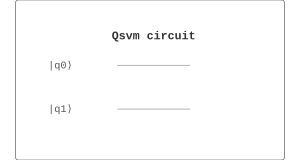
\includegraphics[width=0.6\textwidth]{../../images/qsvm_circuit.svg}
\end{center}

\subsection{数学推导}

量子核函数：
\begin{equation}
K(x_i, x_j) = |\langle\phi(x_i)|\phi(x_j)\rangle|^2
\end{equation}

\subsection{几何解释}

量子 SVM 在量子态空间中分类数据。

\section{代码详解}

\begin{verbatim}
from quonic.ml import qsvm

# qsvm(data, labels)
# data: input data
# labels: target labels
result = qsvm(data=[[0,1],[1,0]], labels=[0,1])
print(f'Accuracy: {result.accuracy}')
\end{verbatim}

\section{进阶用法}

\subsection{场景 1：不同数据}

\begin{verbatim}
from quonic.ml import qsvm
result = qsvm(data=[[0,1],[1,0],[1,1]], labels=[0,1,1])
print(f'Accuracy: {result.accuracy}')
\end{verbatim}

\section{适用场景}

\subsection{分类}

量子 SVM 可以用于分类问题。

\subsection{模式识别}

量子 SVM 可以用于模式识别。

\section{常见问题}

\subsection{量子 SVM 的优势是什么？}

可以在高维特征空间中分类。

\subsection{量子 SVM 的精度如何？}

取决于核函数的选择。

\section{学习路径}

\subsection{前置知识}
\begin{itemize}
  \item 量子核方法
  \item 支持向量机
  \item 量子机器学习
\end{itemize}

\subsection{继续学习}
\begin{itemize}
  \item 量子分类
  \item 量子模式识别
  \item 量子机器学习
\end{itemize}

\section{完整示例代码}

\subsection{示例 1：基本量子 SVM}

\begin{verbatim}
from quonic.ml import qsvm
result = qsvm(data=[[0,1],[1,0]], labels=[0,1])
print(f'Accuracy: {result.accuracy}')
\end{verbatim}

\section{下载}

\begin{itemize}
  \item [qsvm.py](https://github.com/ChrisLee0721/QuoNic/blob/main/examples/qsvm/qsvm.py)
\end{itemize}

\end{document}
